\documentclass{article}
\usepackage[utf8]{inputenc}
\usepackage{fancyhdr,graphicx,parskip}
\usepackage[margin=1in]{geometry}
\renewcommand{\headrulewidth}{0pt}
\fancyhead[R]{\includegraphics[width=3.5cm]{logdep.PNG}}
\fancyhead[L]{\includegraphics[width=2.5cm]{escup.PNG}
}

\graphicspath{ {images/} }
\usepackage{vmargin}
\usepackage{amsmath}
\usepackage{graphicx}
\usepackage[spanish]{babel}
\usepackage[utf8]{inputenc}
\usepackage[spanish]{babel}
\usepackage{afterpage}
\usepackage{subfigure}
\usepackage{hyperref}
\usepackage{cancel}
\usepackage{txfonts} 
\usepackage{pxfonts}
\usepackage{multicol}


\title{ }
\author{\\ L. MELISSA NIÑO VERA   CC. 109427637 \\  Universidad de Pamplona \\ Programa de Física \\ Materia }


\begin{document}
\maketitle
\thispagestyle{fancy}

\begin{center}
    \section*{GRÁFICA: LONGITUD DE ONDA DE ESTRELLAS VS DISTANCIA}
\end{center}

\section{INTRODUCCIÓN}

El estudio de las estrellas es fundamental para comprender la estructura y evolución del universo. Las propiedades de estos cuerpos celestes, como su temperatura, color y distancia, están estrechamente relacionadas y pueden analizarse mediante herramientas computacionales.

En este trabajo, se presenta un análisis de la longitud de onda predominante de diversas estrellas en función de su distancia a la Tierra. Para ello, se ha implementado un código en Python que, en su primera parte, intenta consultar información astronómica desde la base de datos SIMBAD a través de la librería astroquery.simbad. Sin embargo, esta consulta no se llevó a cabo correctamente debido a posibles problemas de conexión o configuración.

En la segunda parte del código, se definen los datos de varias estrellas con sus respectivas distancias y longitudes de onda, permitiendo su visualización en un gráfico de dispersión. La representación gráfica utiliza colores para indicar la temperatura de las estrellas, siguiendo la relación establecida por la ley de Wien, que vincula la longitud de onda de máxima emisión con la temperatura superficial de un cuerpo estelar.

Este análisis proporciona una manera visual e intuitiva de entender cómo la temperatura y la distancia de las estrellas están interconectadas, ofreciendo una herramienta útil para el estudio de la física estelar y la evolución astronómica.

\section{GRÁFICA}

 \begin{figure}[h!]
        \begin{center}
        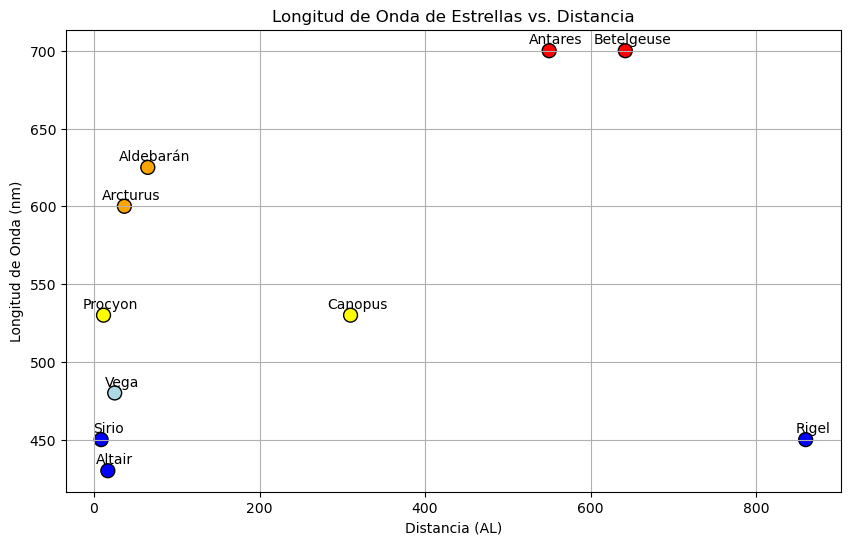
\includegraphics[width=4.5in]{longitudes de onda.png}
            \caption{Relación entre la distancia de las estrellas y la longitud de onda visible.}
            \label{fig1}
        \end{center}
    \end{figure}
    
La gráfica presentada \ref{fig1} muestra la relación entre la longitud de onda predominante de la luz emitida por diversas estrellas y su distancia en años luz (AL) respecto a la Tierra. La longitud de onda está relacionada con la temperatura de la estrella, mientras que la distancia nos indica cuán lejos está el objeto en el cosmos. Este análisis examina el significado físico de la distribución de las estrellas en el gráfico y cómo se correlacionan la temperatura, el color y la distancia.

\section{RELACIÓN ENTRE LAS VARIABLES}
\subsection{Relación entre Longitud de Onda y Temperatura}

De acuerdo con la ley de Wien, la longitud de onda de la emisión máxima de un cuerpo negro está inversamente relacionada con su temperatura:

\[ \lambda_{max} = \frac{b}{T} \]

Donde \( \lambda_{max} \) es la longitud de onda del pico de emisión en metros, \( b \) es la constante de desplazamiento de Wien $(2.897 \times 10^{-3} m\cdot K) $ y \( T \) es la temperatura en kelvins.

En la gráfica, observamos que las estrellas con longitudes de onda menores (azules/blancas) tienen temperaturas más altas. Ejemplos incluyen Sirio, Vega y Rigel. Estrellas con longitudes de onda mayores (rojizas) son más frías. Ejemplos incluyen Betelgeuse y Antares. Estrellas intermedias (blanco-amarillo y naranja) tienen temperaturas moderadas. Ejemplos incluyen Procyon, Canopus y Aldebarán.

\subsection{Relación entre Distancia y Tipo Espectral} 

Si bien no hay una relación directa entre la distancia y la longitud de onda en esta gráfica, se puede concluir que algunas de las estrellas más frías y rojas, como Betelgeuse y Antares, son supergigantes rojas y se encuentran a distancias de cientos de años luz; las estrellas calientes como Sirio y Altair son relativamente cercanas. Rigel, una estrella azul-blanca muy caliente, está entre las más lejanas en el gráfico, lo que indica que es una estrella masiva y brillante.

\subsection{Clasificación Espectral y Evolución Estelar}

Las estrellas pueden clasificarse según su tipo espectral, que está relacionado con la temperatura:

\begin{itemize}
    \item O y B son azules, calientes y longevidad corta, como por ejemplo: Rigel.
    \item A y F son blanco-azul y blanco-amarillo con  temperaturas intermedias, como por ejemplo  Sirio, Vega, Canopus, Procyon.
    \item G, K son amarillas y naranjas, estrellas de secuencia principal y gigantes, como por ejemplo Arcturus.
    \item M son rojas, frías, gigantes o enanas, como por ejemplo Betelgeuse y Antares.
\end{itemize}

Las estrellas más masivas evolucionan rápidamente y se convierten en supergigantes, mientras que las menos masivas, como el Sol, evolucionan más lentamente hacia la fase de gigante roja.

\section{CONCLUSIÓN:}

La gráfica ilustra la relación entre la temperatura superficial de las estrellas (a través de la longitud de onda predominante) y su distancia. Se observa que las estrellas calientes tienden a tener longitudes de onda menores (colores azulados), mientras que las estrellas frías presentan longitudes de onda mayores (colores rojizos). Además, la distribución de las estrellas en términos de distancia refleja diferentes etapas en la evolución estelar y su brillo intrínseco. Este tipo de análisis es fundamental para comprender la estructura y evolución del universo.



\end{document}
